\documentclass[tikz,border=2pt]{standalone}
\usepackage{amsmath,amssymb}
\usepackage{tikz}
\usetikzlibrary{arrows.meta}

\begin{document}
% Corner points: feasible intersections of two constraint boundaries (n = 2 independent
% boundary equations). The polygon has five of them.
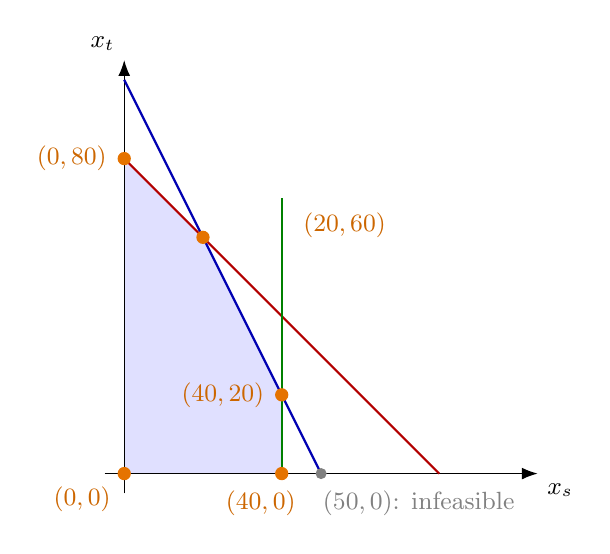
\begin{tikzpicture}[x=0.05cm, y=0.05cm, every node/.style={font=\small}, >={Latex[length=2mm]}]
	\fill[blue!12] (0,0) -- (40,0) -- (40,20) -- (20,60) -- (0,80) -- cycle;
	\draw[->] (-5,0) -- (105,0) node[below right] {$x_s$};
	\draw[->] (0,-5) -- (0,105) node[above left] {$x_t$};
	\draw[blue!70!black, thick] (50,0) -- (0,100);
	\draw[red!70!black, thick] (80,0) -- (0,80);
	\draw[green!50!black, thick] (40,0) -- (40,70);
	\foreach \p in {(0,0),(40,0),(40,20),(20,60),(0,80)} {\fill[orange!90!black] \p circle (2.4pt);}
	\node[orange!80!black, font=\small, anchor=north east] at (-1,-1) {$(0,0)$};
	\node[orange!80!black, font=\small, anchor=north east] at (46,-2) {$(40,0)$};
	\node[orange!80!black, font=\small, anchor=east] at (38,20) {$(40,20)$};
	\node[orange!80!black, font=\small, anchor=west] at (43,63) {$(20,60)$};
	\node[orange!80!black, font=\small, anchor=east] at (-2,80) {$(0,80)$};
	\fill[gray] (50,0) circle (2pt);
	\node[gray, font=\small, anchor=north west] at (48,-2) {$(50,0)$: infeasible};
	\end{tikzpicture}
\end{document}
